\label{sec:methodology}

\subsection{Vision-Language Models Evaluated}

We evaluate 16 state-of-the-art VLMs across six major model families, with parameters ranging from 256M to 8.3B. The models represent diverse architectural approaches to multimodal understanding:

\begin{itemize}
    \item \textbf{Qwen Family}: Qwen2.5-VL-3B, Qwen2.5-VL-7B, Qwen2-VL-2B
    \item \textbf{SmolVLM Family}: SmolVLM2-256M, SmolVLM2-500M, SmolVLM2-2.2B
    \item \textbf{InternVL Family}: InternVL3-1B, InternVL3-2B, InternVL2.5-4B
    \item \textbf{LLaVA Family}: LLaVA-1.5-7B, LLaVA-v1.6-Mistral-7B
    \item \textbf{DeepSeek Family}: DeepSeek-VL-1.3B, DeepSeek-VL-7B
    \item \textbf{Others}: Moondream2-2B, Gemma-3-4B-IT, PaliGemma-3B
\end{itemize}

These models span different size categories: (0-1]B, (1-2]B, (2-3]B, (3-4]B, and (6-7]B parameters, enabling analysis of scale-robustness relationships.

\subsection{Epsilon-Based Attack Framework}

We introduce a novel epsilon-based attack framework that provides direct perturbation control without requiring optimization. This approach ensures consistent perturbation bounds across different attack types and models, enabling fair comparison of robustness characteristics.

\subsubsection{Perturbation Constraint}

All adversarial examples $x'$ are constrained by the $L_\infty$ norm:
\begin{equation}
\|x' - x\|_\infty \leq \epsilon
\end{equation}

where $x$ is the original image and $\epsilon$ represents the maximum allowed perturbation magnitude. We evaluate three epsilon levels:
\begin{itemize}
    \item \textbf{Subtle}: $\epsilon = 0.02$ (small perturbations)
    \item \textbf{Moderate}: $\epsilon = 0.05$ (medium perturbations)
    \item \textbf{Strong}: $\epsilon = 0.08$ (large perturbations)
\end{itemize}

\subsubsection{White-Box Attacks}

\textbf{Fast Gradient Sign Method (FGSM)} \cite{goodfellow2014explaining}: The fundamental single-step attack computes adversarial examples as:
\begin{equation}
x' = x + \epsilon \cdot \text{sign}(\nabla_x J(\theta, x, y))
\end{equation}
where $J(\theta, x, y)$ is the loss function, $\theta$ represents model parameters, and $y$ is the true label.

\textbf{Projected Gradient Descent (PGD)} \cite{madry2017towards}: An iterative extension of FGSM that performs multiple gradient steps with projection:
\begin{equation}
x'^{(t+1)} = \Pi_{x+S} \left( x'^{(t)} + \alpha \cdot \text{sign}(\nabla_x J(\theta, x'^{(t)}, y)) \right)
\end{equation}
where $\Pi_{x+S}$ projects onto the $L_\infty$ ball of radius $\epsilon$ around $x$, and $\alpha = \epsilon/T$ with $T$ iterations.

\textbf{Auto Projected Gradient Descent (AutoPGD)} \cite{croce2020reliable}: An parameter-free variant of PGD that automatically adapts step sizes:
\begin{equation}
x'^{(t+1)} = \Pi_{x+S} \left( x'^{(t)} + \alpha_t \cdot \text{sign}(\nabla_x J(\theta, x'^{(t)}, y)) \right)
\end{equation}
where $\alpha_t$ is adaptively chosen based on attack progress.

\textbf{Auto Conjugate Gradient} \cite{yamamura2022auto}: Applies conjugate gradient optimization to adversarial example generation:
\begin{equation}
x'^{(t+1)} = x'^{(t)} + \beta_t d_t
\end{equation}
where $d_t$ is the conjugate direction and $\beta_t$ is computed using the Polak-Ribière formula.

\textbf{Basic Iterative Method (BIM)} \cite{kurakin2016adversarial}: An iterative approach with smaller step sizes:
\begin{equation}
x'^{(t+1)} = \text{Clip}_{x,\epsilon} \left( x'^{(t)} + \alpha \cdot \text{sign}(\nabla_x J(\theta, x'^{(t)}, y)) \right)
\end{equation}
where $\text{Clip}_{x,\epsilon}$ ensures the result stays within the $L_\infty$ ball.

\subsubsection{Black-Box Attacks}

\textbf{Square Attack} \cite{andriushchenko2020square}: A query-efficient attack that randomly samples square-shaped perturbations:
\begin{equation}
x' = x + \delta
\end{equation}
where $\delta$ is sampled from square-shaped regions with probability $p_{init}$ and magnitude bounded by $\epsilon$.

\textbf{SimBA} \cite{guo2019simple}: Simple black-box attack using coordinate-wise perturbations:
\begin{equation}
x'^{(t+1)} = x'^{(t)} + \epsilon \cdot e_i \cdot \text{sign}(\Delta_i)
\end{equation}
where $e_i$ is the $i$-th coordinate vector and $\Delta_i$ measures the change in model output.

\textbf{Boundary Attack} \cite{brendel2017decision}: Decision-based attack that starts from adversarial examples and moves toward the decision boundary:
\begin{equation}
x'^{(t+1)} = x'^{(t)} + \delta \cdot \frac{\nabla \hat{f}(x'^{(t)})}{\|\nabla \hat{f}(x'^{(t)})\|}
\end{equation}
where $\hat{f}$ is the estimated decision function and $\delta$ controls step size.

\textbf{SignOPT} \cite{cheng2019sign}: Hard-label attack optimizing the sign of gradients:
\begin{equation}
x'^{(t+1)} = x'^{(t)} + \beta \cdot \text{sign}(\hat{g}_t)
\end{equation}
where $\hat{g}_t$ is the estimated gradient using finite differences and $\beta$ is the step size.

\subsection{System Architecture}

Our adversarial robustness evaluation framework follows a modular design pattern that enables systematic assessment of VLM vulnerabilities across diverse attack scenarios. The architecture comprises six interconnected components that collectively form a comprehensive evaluation pipeline.

\subsubsection{Component Architecture and Data Flow}

\textbf{Adversarial Attack Orchestration Framework}: The central coordinator that manages the execution of all attack scenarios. This component interfaces with specialized attack generation modules and ensures consistent parameter control across different epsilon levels and attack types. It implements batch processing capabilities and maintains execution state for reproducible experiments.

\textbf{Attack Generation Modules}: Two specialized frameworks handle different attack paradigms:
\begin{itemize}
    \item \textbf{White-Box Attack Generation Module}: Implements gradient-based attacks (FGSM, PGD, AutoPGD, AutoConjugateGradient, BasicIterativeMethod) with direct access to model parameters and gradients
    \item \textbf{Black-Box Attack Generation Module}: Implements query-based attacks (Square, SimBA, Boundary, SignOPT) that require only model outputs
\end{itemize}

\textbf{Shared Computational Library}: Provides common utilities including GPU-optimized computations using Numba JIT compilation, image preprocessing pipelines, epsilon calculation in normalized [0,1] space, and PyTorch classifier creation with memory management.

\textbf{VLM Interface Layer}: Abstracts model access through two specialized interfaces:
\begin{itemize}
    \item \textbf{Local Model Interface}: Thread-safe management of 16 local VLM models with automatic memory optimization and model caching
    \item \textbf{Cloud API Interface}: Standardized access to cloud-based models (GPT-4V) with retry mechanisms and rate limiting
\end{itemize}

\textbf{Experimental Data Management System}: Centralized SQLite database that replaces traditional JSON-based approaches, ensuring ACID compliance, transaction safety, and efficient data access. Manages attack parameters, inference results, ground truth data, and performance metrics.

\textbf{Evaluation and Analytics Pipeline}: Comprises three specialized modules:
\begin{itemize}
    \item \textbf{VLM Inference Pipeline}: Coordinates model evaluation across clean and adversarial images with comprehensive performance monitoring
    \item \textbf{Robustness Assessment Engine}: Implements multi-method evaluation including numerical accuracy (±5\% tolerance), ROUGE-L scoring, exact matching, and semantic similarity analysis
    \item \textbf{Performance Analytics and Visualization Module}: Generates publication-ready visualizations and statistical analyses including baseline comparisons, attack effectiveness heatmaps, and architecture vulnerability assessments
\end{itemize}

\subsubsection{Data Flow Architecture}

The evaluation pipeline follows a systematic data flow illustrated in the architecture diagram below:

\begin{verbatim}
                  +---------------------+
                  | Attack Orchestration| ---+
                  | Framework           |    |
                  +---------------------+    |
                                             V
              +-----------------+   +-----------------+
              | White-Box Attack|   | Black-Box Attack|
              | Generation      |   | Generation      |
              +-----------------+   +-----------------+
                       |                      |
                       +----------+-----------+
                                  V
                       +---------------------+
                       | Shared Computational|
                       | Library             |
                       +---------------------+
                                  |
                                  V
                       +---------------------+
                       | Experimental Data   |
                       | Management System   |
                       +---------------------+
                                  |
                                  V
                       +---------------------+
                       | VLM Inference       |
                       | Pipeline            |
                       +---------------------+
                                  |
                          +-------+-------+
                          V               V
                  +-------------+ +-------------+
                  |Local Model  | |Cloud API    |
                  |Interface    | |Interface    |
                  +-------------+ +-------------+
                          |               |
                          +-------+-------+
                                  V
                       +---------------------+
                       | Robustness Assessment|
                       | Engine              |
                       +---------------------+
                                  |
                                  V
                       +---------------------+
                       | Performance Analytics|
                       | & Visualization     |
                       +---------------------+
\end{verbatim}

The systematic data flow operates through five distinct stages:
\begin{enumerate}
    \item \textbf{Input Stage}: Original images and ground truth questions are processed through the Experimental Data Management System
    \item \textbf{Attack Generation Stage}: The Adversarial Attack Orchestration Framework coordinates attack generation using specialized modules and shared utilities
    \item \textbf{Model Evaluation Stage}: Clean and adversarial images are processed through the VLM Interface Layer using the Inference Pipeline
    \item \textbf{Assessment Stage}: The Robustness Assessment Engine evaluates model responses against ground truth using multiple methodologies
    \item \textbf{Analysis Stage}: The Performance Analytics Module generates comprehensive visualizations and statistical summaries
\end{enumerate}

\subsection{Vision-Language Task Evaluation}

We evaluate robustness across 8 diverse vision-language tasks designed to test different aspects of multimodal understanding. Figure~\ref{fig:task_examples} illustrates representative examples from each task category, showing the diversity of visual reasoning challenges in our evaluation framework.

\begin{figure*}[!t]
\centering
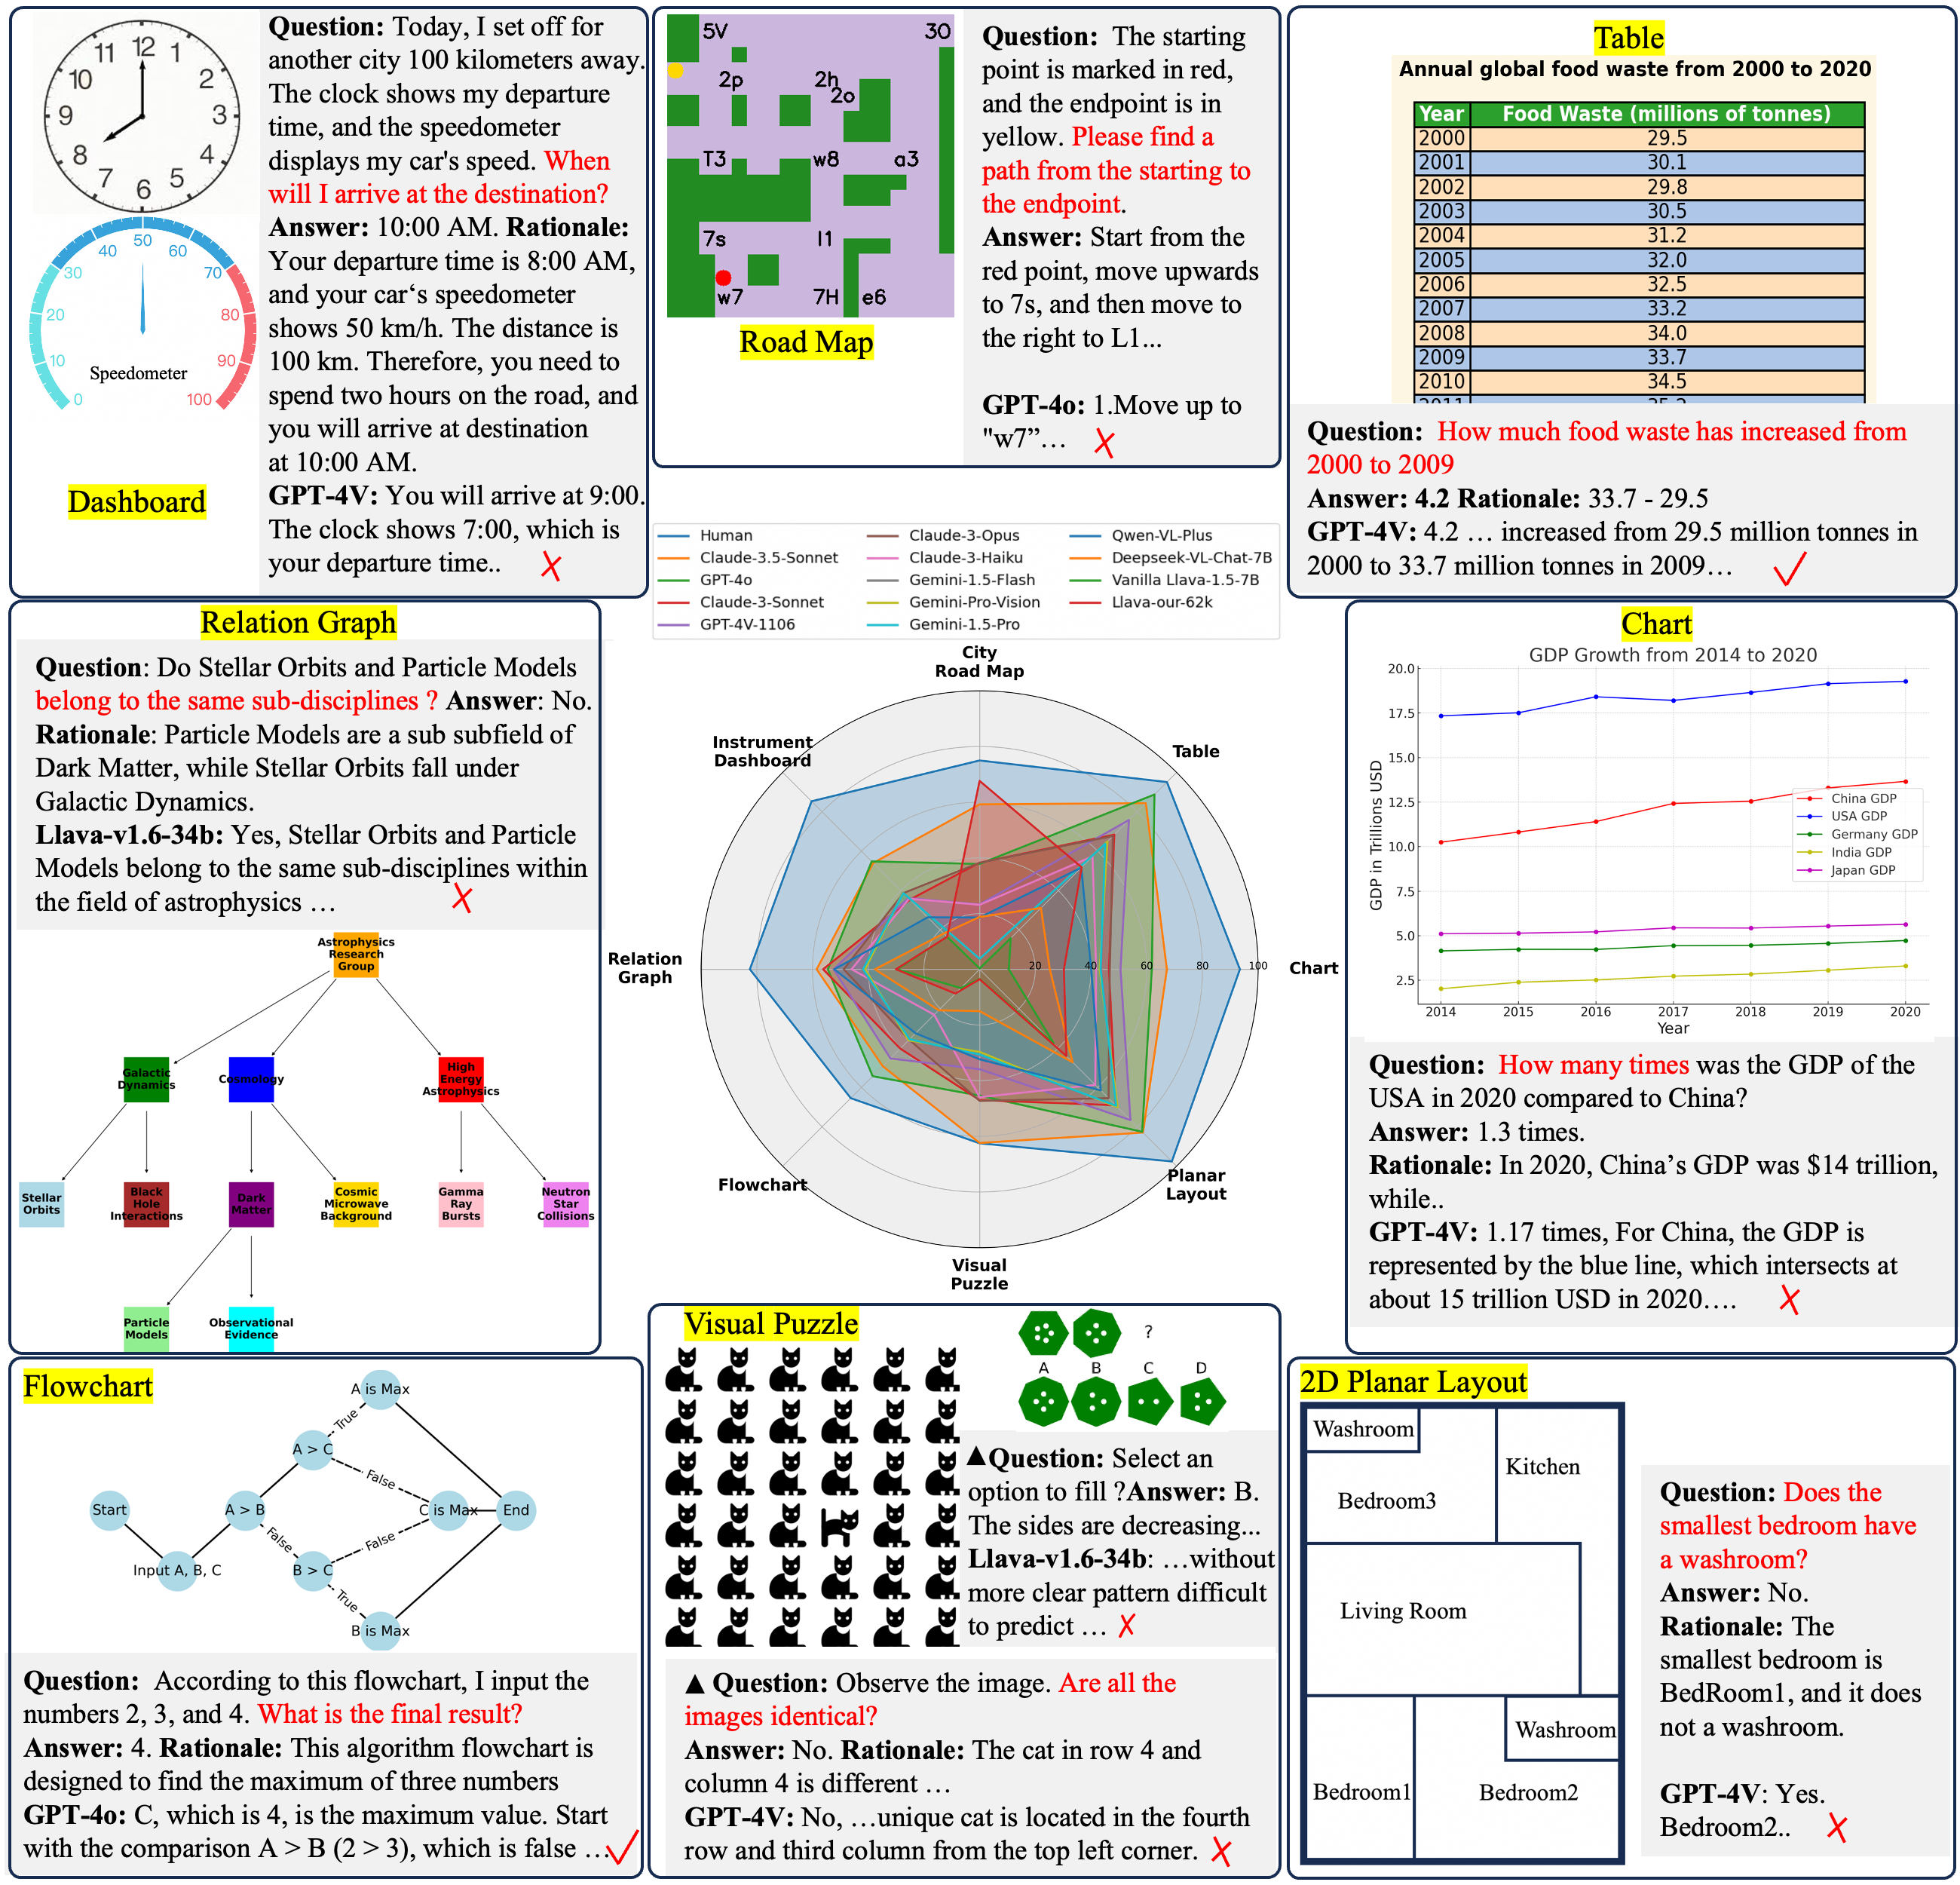
\includegraphics[width=0.9\textwidth]{figure1_final.png}
\caption{Representative examples of the 8 vision-language task categories used in our robustness evaluation. Each task tests different aspects of multimodal understanding: Dashboard (temporal reasoning with analog displays), Road Map (spatial navigation and route planning), Table (structured data interpretation), Relation Graph (network topology understanding), Chart (quantitative data extraction), Flowchart (logical process flow), Visual Puzzle (pattern recognition and completion), and Planar Layout (spatial arrangement reasoning).}
\label{fig:task_examples}
\end{figure*}

The evaluation tasks are categorized as follows:

\begin{enumerate}
    \item \textbf{Chart Interpretation}: Extracting quantitative information from bar charts, line graphs, and pie charts
    \item \textbf{Table Extraction}: Reading and understanding structured tabular data
    \item \textbf{Road Map Navigation}: Spatial reasoning and route planning from map images
    \item \textbf{Dashboard Analysis}: Interpreting complex multi-widget interfaces
    \item \textbf{Flowchart Understanding}: Following logical flow and decision trees
    \item \textbf{Relation Graph Analysis}: Understanding node-edge relationships
    \item \textbf{Planar Layout Interpretation}: Spatial arrangement and geometric reasoning
    \item \textbf{Visual Puzzle Solving}: Pattern recognition and logical reasoning
\end{enumerate}

Each task includes multiple question types: numerical extraction, multiple-choice, and open-ended summarization, enabling comprehensive evaluation of different reasoning capabilities.

\subsection{Evaluation Metrics}

\textbf{Accuracy Calculation}: For each model-attack-task combination, we compute:
\begin{equation}
\text{Accuracy} = \frac{\text{Number of Correct Responses}}{\text{Total Number of Questions}}
\end{equation}

\textbf{Robustness Measurement}: The primary robustness metric is accuracy degradation:
\begin{equation}
\text{Accuracy Change} = \text{Accuracy}_{\text{adversarial}} - \text{Accuracy}_{\text{clean}}
\end{equation}

Negative values indicate performance degradation under adversarial perturbations.

\textbf{Response Evaluation}: We employ multiple evaluation methodologies depending on question type:
\begin{itemize}
    \item \textbf{Numerical}: ±5\% tolerance for quantitative answers
    \item \textbf{ROUGE-L}: For summary-type responses using Lin's ROUGE package \cite{lin2014rouge}
    \item \textbf{Exact Match}: For multiple-choice and categorical responses
    \item \textbf{Semantic Similarity}: Using WordNet \cite{miller1995wordnet} for synonym matching
\end{itemize}

\subsection{Attack Success Criteria}

An attack is considered successful if:
\begin{enumerate}
    \item The adversarial perturbation satisfies $\|x' - x\|_\infty \leq \epsilon$
    \item The model's response changes from correct to incorrect
    \item The achieved epsilon is within 10\% tolerance of the target epsilon
\end{enumerate}

This ensures that successful attacks produce meaningful perturbations that actually affect model performance rather than simply generating noisy images.